%%%%%%%%%%%%Outline%%%%%%%%%%%%%%%%%%

%%%
% message<we evaluate \sys with three questions, each taking different evidence>
% we evaluate \sys with three questions
% RQ1 asks whether the diagnostic is a more actionable basis for repair than the raw log
% RQ2 asks what the diagnostic adds over the verifier message
% RQ3 asks whether \sys identifies the layer when several layers share a message

%%%
% message<two datasets: bpfix-bench repair tasks with oracles for RQ1, bpfix-empirical labeled rejections for RQ2 and RQ3>
% we use two datasets
% bpfix-bench is 75 repair tasks, 40 proof-obligation and 35 from open-source projects (Cilium, xdp-tools, bpftime), each with an oracle
% bpfix-empirical is the 235 reproduced rejections from section 2, each with a hand-assigned layer
% RQ1 runs on bpfix-bench, RQ2 and RQ3 on bpfix-empirical

%%%
% message<we test whether the diagnostic enables more repairs than the raw log, judged by an oracle independent of \sys>
% we test whether more rejected programs can be repaired from the diagnostic than from the raw log
% we give a language model the buggy program with one of the two inputs, and it writes a candidate fix
% an oracle independent of \sys accepts a fix only if the program loads through the verifier and passes the case's tests
% we score each task at one shot and after one failure-informed retry, to test the diagnostic alone and whether the help persists
% the primary model is Qwen3.6 27B, with the hosted GLM 5.2 and a small Qwen2.5 3B, at temperature zero
% the 3B shows whether the gain depends on model capacity

%%%
% message<the diagnostic raises repair under every model, so the gain comes from the diagnostic>
% replacing the raw log with the diagnostic raises repair under every model
% on 27B 22 from raw and 38 from the diagnostic one-shot, 30 vs 44 with retry
% GLM agrees 28 to 38, the retry narrows the gap 47 to 52
% the 3B repairs 0 from raw and 8 from the diagnostic one-shot, 10 with retry
% the gain holds under three models, so it comes from the diagnostic

%%%
% message<the diagnostic removes verifier-load and source-semantics failures, helping the model satisfy the verifier and keep behavior>
% we charge each failed candidate to the first stage it fails: return, compile, verifier-load, functional, source-semantics
% the diagnostic mainly removes verifier-load and source-semantics failures, 19 to 10 and 22 to 16 on 27B
% so it helps the model satisfy the verifier and preserve behavior
% the 3B model-call failures are a length effect from raw prompts overflowing its context

%%%
% message<RQ2 measures what the diagnostic adds over the bare message: the four repair fields it supplies>
% the bare message names only the failing operation, but a repair needs more
% RQ2 measures what the \sys diagnostic adds
% we run \sys on all 235 rejections and record which of four repair fields each diagnostic supplies, against the message

%%%
% message<every diagnostic supplies the four fields the message lacks, on the development corpus>
% every diagnostic supplies all four fields, the message none
% an example shows the terminal line giving only the symptom while \sys adds all four
% \sys produces a supported diagnostic for every corpus rejection across 21 families, though the corpus guided its development

%%%
% message<we find messages that span multiple layers and judge separation on the largest collision, grounded in upstream fixes>
% a repair must change the right layer, yet one message can carry more than one
% we search for messages spanning more than one layer and study the largest collision
% the ground truth for each compiler case is the upstream build-level fix, independent of \sys
% we compare \sys against a message dictionary and count correct assignments, as a case study

%%%
% message<the dictionary collapses the scalar collision to source bugs while \sys separates the lowering cases>
% the scalar message reaches bpfix-empirical 28 times, 24 source bugs and four lowering artifacts
% the dictionary labels all 28 source bugs and recovers none of the four lowering cases
% \sys reads where pointer provenance is lost and flags the four without mislabeling the source bugs
% the ground truth is the upstream fix, which \sys did not produce
% the false-positive layer is hardest to ground, so this study covers only lowering against source

%%%
% message<threats: working suite, label co-development, localization, small classes, one environment>
% bpfix-bench is a working suite, a frozen heldout split is future work
% every number comes from one pinned kernel and compiler, verifier behavior is version-specific
% the bpfix-empirical class labels were developed alongside \sys, so we do not report accuracy against them
% the fix site lies within 13 instructions of the rejected line, so \sys contributes through its diagnostic
% the lowering and false-positive classes carry few cases, reported as raw counts

%%%%%%%%%%%%Outline%%%%%%%%%%%%%%%%%%

\section{Evaluation}
\label{sec:evaluation}

We evaluate \sys with three questions:
\begin{itemize}
  \item \textbf{RQ1.} Is the \sys diagnostic a more actionable basis for repair than the raw verifier log?
  \item \textbf{RQ2.} Does the \sys diagnostic supply the repair information the verifier message omits?
  \item \textbf{RQ3.} Can \sys identify the responsible layer when several layers share one verifier message?
\end{itemize}

\noindent\textbf{Datasets.} We use two datasets. \bench holds 75 source-level repair tasks, 40 built around a verifier proof obligation and 35 minimized from open-source projects such as Cilium~\cite{cilium}, xdp-tools~\cite{xdptools}, and bpftime~\cite{zheng2025extending}, and each task ships the buggy program with an executable oracle. \empiricalset holds the 235 reproduced rejections from \S\ref{sec:study:corpus}, each carrying a hand-assigned responsibility layer. RQ1 runs on \bench, and RQ2 and RQ3 run on \empiricalset. 
% \xiangyu{Add reference to \bench and \empiricalset. Additionally, do we have baseline to compare?} 

\noindent\textbf{RQ1: Repair effectiveness.} We test whether more rejected programs can be repaired from the \sys diagnostic than from the raw verifier log. We give a language model the buggy program with either the raw log or the \sys diagnostic, and the model writes a candidate fix. An executable oracle independent of \sys accepts a fix only if the program loads through the kernel verifier and passes the case's functional and source-semantics tests. We score each task at one shot, to test the diagnostic on its own, and after one failure-informed retry, to test whether the help persists. Our primary model is Qwen3.6 27B, and we also run the hosted GLM 5.2 and a small Qwen2.5 3B at temperature zero. The 3B shows whether the gain depends on model capacity. 

Replacing the raw log with the \sys diagnostic raises repair under every model (Figure~\ref{fig:bpfix-bench}). On Qwen3.6 27B, the model repairs 22 of the 75 cases from the raw log in one shot and 38 from the diagnostic, and one retry raises the two to 30 and 44. GLM 5.2 shows the same one-shot gain, 28 against 38, though the retry narrows the gap, 47 against 52. The small Qwen2.5 3B repairs none of the 75 from the raw log, and 8 from the diagnostic in one shot and 10 with one retry. Because the gain holds under three different models, it comes from the diagnostic.
% \xiangyu{Is it OK to say that we can get similar results if we use other language models? If this is the case, we should say that.}
\begin{figure}[H]
  \centering
  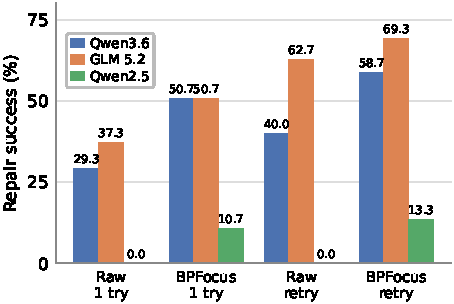
\includegraphics[width=0.9\columnwidth]{figures/sec-5-bpfix-test.pdf}
  \caption{\testset repair success across three models. Bars are grouped by prompt mode and colored by model; retry bars use one failure-informed retry.}
  \label{fig:bpfix-test}
\end{figure}


To locate the gain, we charge each failed candidate to the first stage it fails: returning a program, compiling, loading through the verifier, passing the functional test, or passing the source-semantics test (Table~\ref{tab:failure-stage}). The diagnostic mainly removes verifier-load and source-semantics failures: on the 27B one-shot run, load failures fall from 19 to 10 and source-semantics failures from 22 to 16, while compile failures stay low. The diagnostic therefore helps the model both satisfy the verifier and preserve the program's behavior. The 3B's model-call failures are a length effect: three raw prompts overflowed its context window and returned no program, while the shorter diagnostic stayed within it.

\begin{table}[t]
  \centering
  \caption{Where repairs fail on \testset, by stage, for the one-attempt runs. The \sys diagnostic mainly removes verifier-load (Load) and proof failures; compile and model-call (Call) failures stay low. Each entry counts failing cases at a stage, and pass count plus the row total is 75.}
  \label{tab:failure-stage}
  \small
  \setlength{\tabcolsep}{4pt}
  \begin{tabular}{@{}l l r r r r r@{}}
    \toprule
    Model & Input & Compile & Load & Func. & Proof & Call \\
    \midrule
    Qwen3.6 27B & raw  &  3 & 19 &  9 & 22 & 0 \\
                & \sys &  1 & 10 & 10 & 16 & 0 \\
    GLM 5.2     & raw  &  1 & 10 & 11 & 25 & 0 \\
                & \sys &  1 &  5 &  9 & 22 & 0 \\
    Qwen2.5 3B  & raw  &  7 & 62 &  0 &  3 & 3 \\
                & \sys & 14 & 39 &  6 &  8 & 0 \\
    \bottomrule
  \end{tabular}
\end{table}


\noindent\textbf{RQ2: Diagnostic completeness.} The bare verifier message names only the failing operation, yet a repair needs more (\S\ref{sec:study}). RQ2 measures what the \sys diagnostic adds. We run \sys on each of the 235 \empiricalset rejections and record, against the raw message, which of four repair fields each diagnostic supplies: a stable error id, the rejected source span, the safety proof the verifier needs, and a next action.

Every diagnostic supplies all four fields, where the raw message supplies none. Figure~\ref{fig:diag-example} shows one rejection where the terminal line gives only the symptom and \sys adds all four. \sys produces a supported diagnostic for every rejection in the corpus, across 21 error families, with no fallback, though the same corpus guided \sys's development.

\begin{figure}[t]
  \noindent\textbf{\footnotesize (a) Rejected program, verifier line, and \sys diagnostic}
  \begin{lstlisting}[style=bpfix,language=C,firstnumber=18]
__u64 *raw_map = (__u64 *)&globals; // &globals: the map object pointer
__u64 v = *raw_map;
*raw_map = v + 1;                   // rejected here
  \end{lstlisting}
  \begin{lstlisting}[style=bpflog]
verifier: only read from bpf_array is supported
  \end{lstlisting}
  \begin{lstlisting}[style=bpfdiag]
error[BPFOCUS-E010]: map pointer is accessed as ordinary memory
  = class: source_bug              --> prog.c:20
  = required proof: derive a map-value pointer with the proper
    map helper before reading or writing map contents
  = next action: look up an element, then write through that pointer
  \end{lstlisting}
  \vspace{2pt}
  \noindent\textbf{\footnotesize (b) Fix that follows the diagnostic}
  \begin{lstlisting}[style=bpfix,language=C,numbers=none]
__u32 key = 0;
__u64 *v = bpf_map_lookup_elem(&globals, &key);
if (!v) return 0;
*v += 1;
  \end{lstlisting}
  \caption{A real rejection from the aya project (issue 1002): (a) the rejected program, the verifier's terminal line, and the \sys diagnostic; (b) the developer's fix.}
  \label{fig:diag-example}
\end{figure}


\noindent\textbf{RQ3: Layer attribution.} \sys reports the responsible layer as a best-effort heuristic (\S\ref{sec:design}). The \empiricalset layer labels were developed alongside \sys, so we examine layer separation through a case study on one message that two layers share. The message \texttt{invalid mem access 'scalar'} prints in \empiricalset for both source bugs and compiler-lowering rejections (\S\ref{sec:study}). We study one rejection of each kind, and the compiler-lowering rejection has correct source with an upstream fix that steers the compiler, so its layer holds independent of \sys.

Figure~\ref{fig:layer-attr} shows the two rejections. Both print \texttt{invalid mem access 'scalar'}, yet \sys reports \texttt{source\_bug} for the integer-to-pointer cast in (a) and \texttt{lowering\_artifact} for the correctly bounds-checked packet pointer in (b). The message is identical, so \sys supplies the layer the message leaves out.

\begin{figure}[t]
  \noindent\textbf{\footnotesize (a) Developer source bug (Stack Overflow 56965789)}
  \begin{lstlisting}[style=bpfix,language=C,firstnumber=17]
if (eth->h_proto == bpf_htons(ETH_P_IP)) {
    struct iphdr *iph2 = (void *)(sizeof(*eth) + nh_off); // integer offset, no packet base
    return iph2->protocol;                                // rejected here
}
  \end{lstlisting}
  \begin{lstlisting}[style=bpfdiag]
error[BPFOCUS-E011]: scalar or pkt_end value is used where the verifier requires a real pointer
  = class: source_bug
  = verifier[31]: R1 invalid mem access 'scalar'
  \end{lstlisting}
  \vspace{2pt}
  \noindent\textbf{\footnotesize (b) Compiler-lowering rejection (Stack Overflow 53136145)}
  \begin{lstlisting}[style=bpfix,language=C,firstnumber=263]
if (ipv4_hdr)
    udph = (void *)ipv4_hdr + sizeof(*ipv4_hdr);
else
    udph = (void *)ipv6_hdr + sizeof(*ipv6_hdr);
if (udph + sizeof(struct udphdr) > data_end)  // udph (merged) bounds-checked
    return 1;

dst_port = __constant_ntohs(((struct udphdr *)udph)->dest); // rejected here
  \end{lstlisting}
  \begin{lstlisting}[style=bpfdiag]
error[BPFOCUS-E006]: verifier-visible compiler lowering hides the required proof
  = class: lowering_artifact
  = verifier[229]: R5 invalid mem access 'scalar'
  \end{lstlisting}
  \caption{Two rejections that share the verifier message \texttt{invalid mem access `scalar'} but need fixes in different layers: a source bug (a) and a compiler-lowering artifact (b). Each diagnostic is abridged to its error id, class, and the verifier line it explains.}
  \label{fig:layer-attr}
\end{figure}

